\chapter{Triển khai hệ thống}

Chương này mô tả cách đưa Social Commerce lên môi trường thực tế. Hình~\ref{fig:deploy-chapter-overview} tóm tắt kiến trúc triển khai; bản mô tả chi tiết các lớp thành phần nằm ở chương Thiết kế (Hình~\ref{fig:deployment-diagram}).

\begin{itemize}
    \item \textbf{Frontend}: Vercel (Vite + React + TypeScript).
    \item \textbf{Backend}: Amazon EC2 (Node.js, Express, Socket.IO).
    \item \textbf{Cơ sở dữ liệu}: Neon (PostgreSQL, Prisma).
    \item \textbf{Cache}: Redis (ví dụ Upstash hoặc AWS ElastiCache).
\end{itemize}

\begin{figure}[H]
\centering
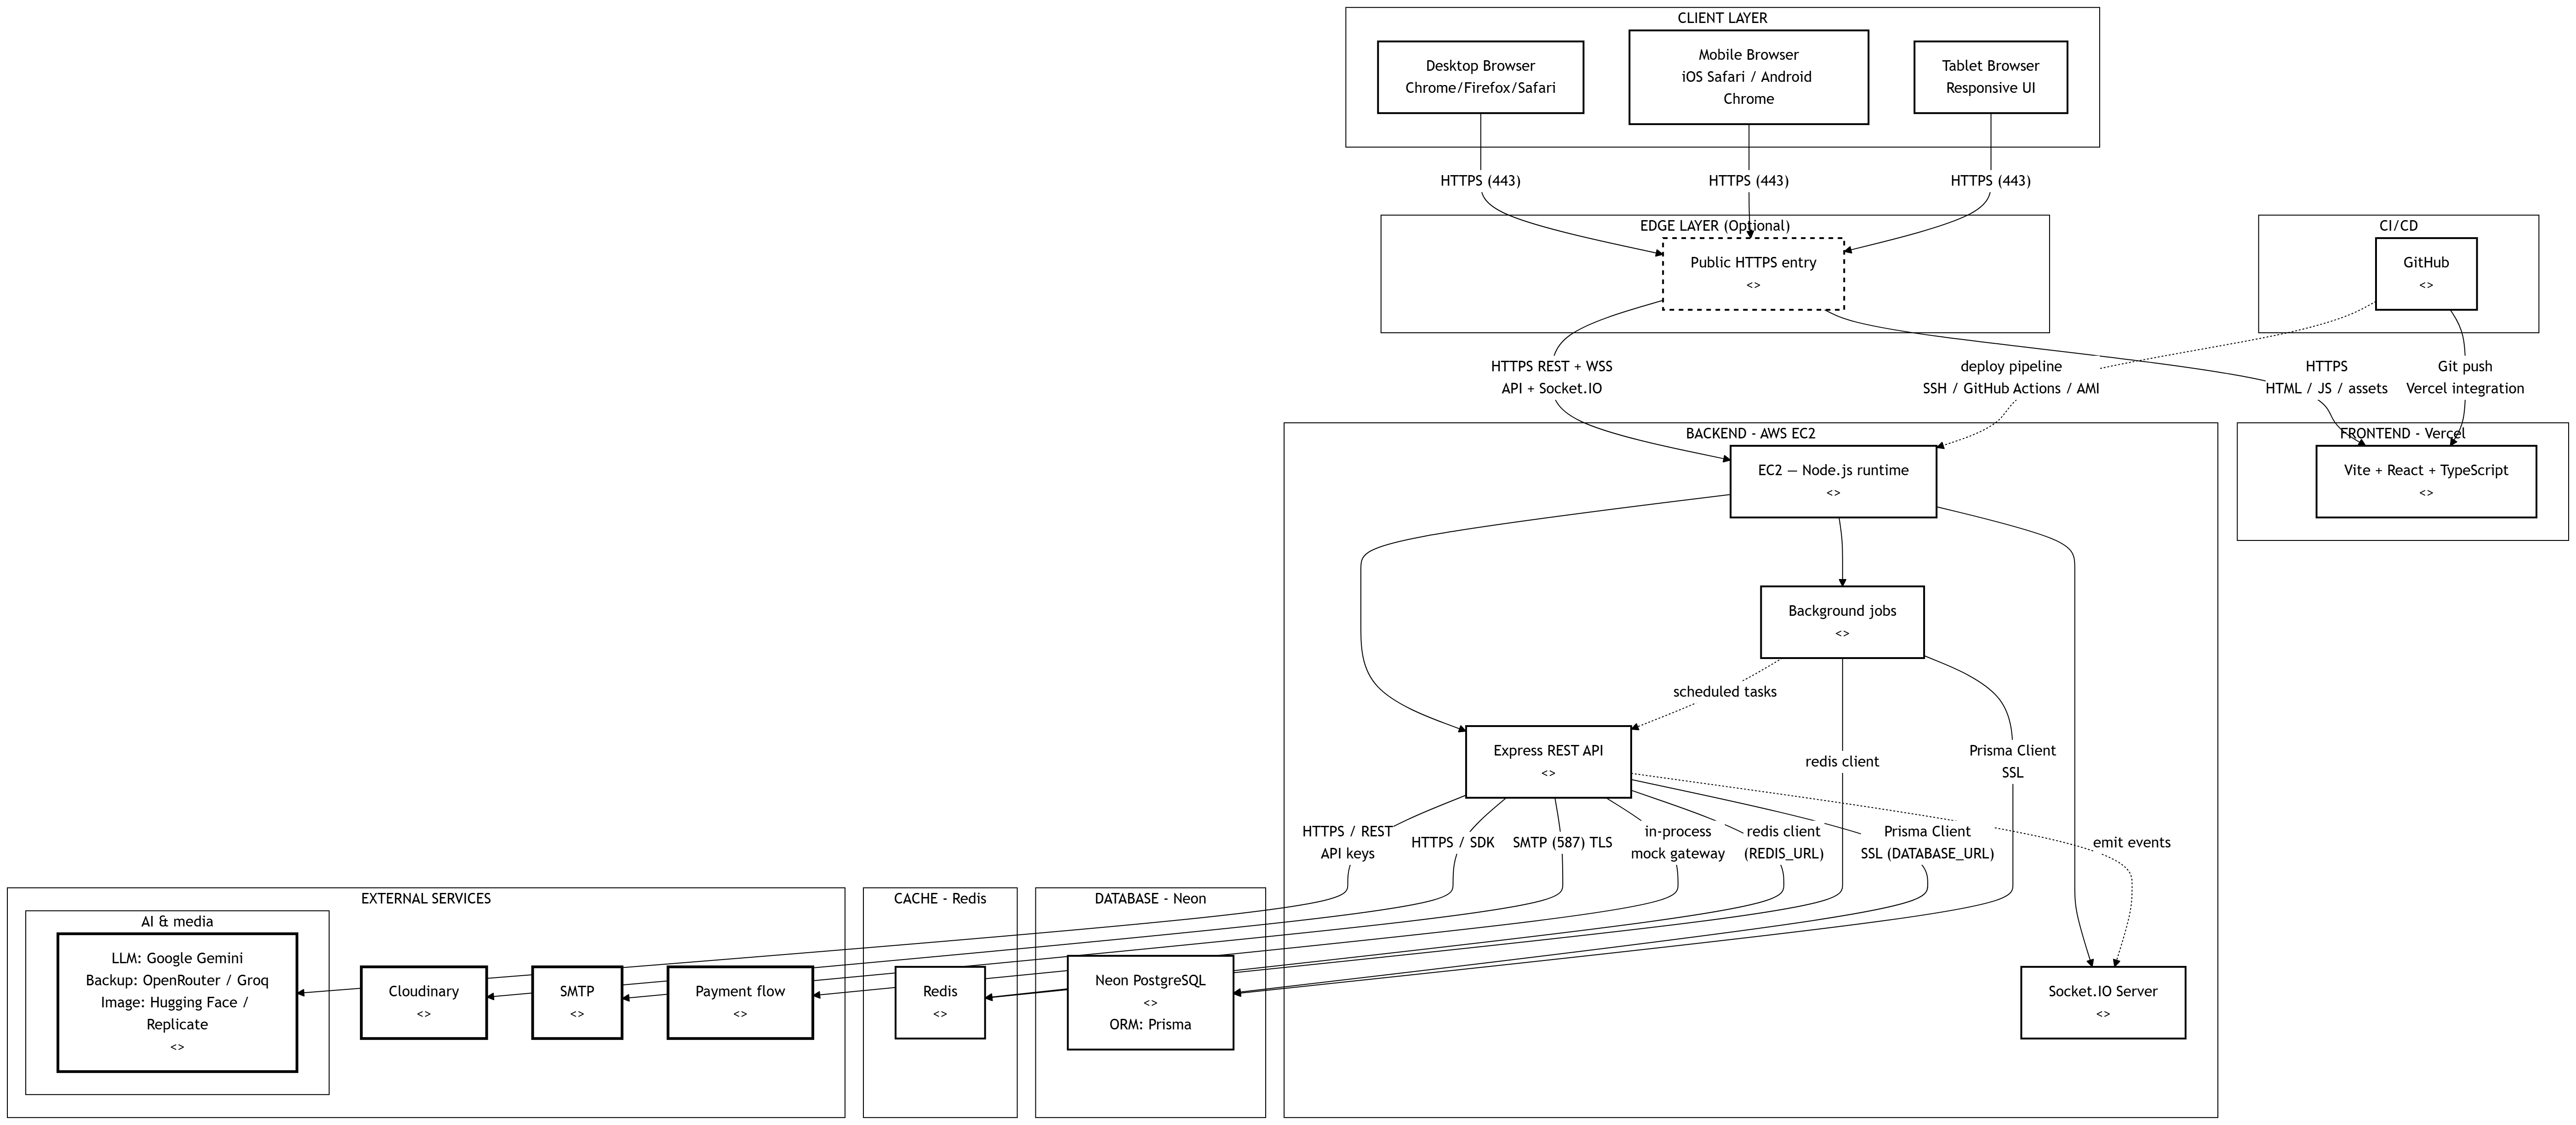
\includegraphics[width=\textwidth]{Images/Deployment Diagram.png}
\caption{Tổng quan kiến trúc triển khai (client, edge, Vercel, EC2, Neon, Redis, dịch vụ ngoài).}
\label{fig:deploy-chapter-overview}
\end{figure}


%----------------------------------------------------------------------
\section{Triển khai cơ sở dữ liệu (Neon) và Redis}
%----------------------------------------------------------------------

\textit{Nên có \texttt{DATABASE\_URL} và \texttt{REDIS\_URL} trước khi cấu hình \texttt{.env} trên EC2.}

\subsection{Neon --- PostgreSQL}

\begin{itemize}
    \item Đăng ký / đăng nhập \href{https://neon.tech}{neon.tech}.
    \item Tạo \textbf{Project} và database mặc định.
    \item Sao chép \textbf{connection string} (PostgreSQL, có SSL) $\rightarrow$ dán vào \texttt{DATABASE\_URL} trong \texttt{backend/.env}.
    \item Trên máy có mạng tới Neon: \texttt{cd backend} $\rightarrow$ \texttt{npm run prisma:generate} $\rightarrow$ \texttt{npm run prisma:migrate:deploy}.
    \item Kiểm tra: Neon SQL Editor hoặc \texttt{npm run prisma:studio} (môi trường dev).
    \item (Tùy chọn) \texttt{npm run prisma:seed} trên môi trường an toàn.
\end{itemize}



\subsection{Redis (cache)}

\begin{itemize}
    \item Tạo database Redis (ví dụ \textbf{Upstash}: copy URL dạng \texttt{rediss://...}; hoặc \textbf{ElastiCache} trong AWS).
    \item Gán \texttt{REDIS\_URL} trong \texttt{backend/.env}.
    \item Khởi động lại tiến trình API (PM2) sau khi đổi biến.
\end{itemize}



%----------------------------------------------------------------------
\section{Triển khai back-end trên Amazon EC2}
%----------------------------------------------------------------------

Stack: \textbf{Ubuntu + Node.js + PM2}; tùy chọn \textbf{Nginx + Certbot} (HTTPS, proxy tới cổng app).

\subsection{Tạo instance EC2}

\begin{itemize}
    \item AWS Console $\rightarrow$ EC2 $\rightarrow$ \textit{Launch instance}.
    \item Chọn AMI \textbf{Ubuntu Server LTS} (x86\_64 hoặc Arm theo instance type).
    \item Chọn instance type (ví dụ \texttt{t3.micro} / \texttt{t2.micro} nếu dùng free tier --- lưu ý giới hạn giờ).
    \item Tạo hoặc chọn \textbf{key pair} (\texttt{.pem}); giữ file private key an toàn.
    \item \textbf{Security group}: mở \textbf{22} (SSH, nên giới hạn IP nếu được), \textbf{80}, \textbf{443} cho HTTP/HTTPS từ Internet (Nginx chấm dứt TLS, proxy về app nội bộ).
    \item Bật \textit{Auto-assign public IP} nếu cần truy cập từ Internet.
    \item Ghi lại \textbf{Public IPv4} hoặc public DNS.
\end{itemize}


\subsection{SSH và cài đặt máy chủ}

\begin{itemize}
    \item Từ máy dev, SSH vào instance (Windows: PowerShell / WSL / Terminal có sẵn \texttt{ssh}).
    \item Ví dụ lệnh (đổi đường key và host):
\begin{lstlisting}[language=bash]
ssh -i "/duong/den/khoa.pem" ubuntu@ec2-xx-xx-xx-xx.ap-southeast-1.compute.amazonaws.com
\end{lstlisting}
    \item Trên server: \texttt{sudo apt update}; cài \texttt{git}.
    \item Cài \textbf{Node.js LTS} (nvm hoặc NodeSource).
    \item Cài PM2: \texttt{sudo npm install -g pm2}.
    \item (Khuyến nghị) Cài \textbf{Nginx} + \textbf{Certbot} $\rightarrow$ chứng chỉ Let's Encrypt cho subdomain \texttt{api.*}; proxy \texttt{443} $\rightarrow$ \texttt{http://127.0.0.1:5000} và bật nâng cấp WebSocket cho Socket.IO.
\end{itemize}

\begin{figure}[H]
\centering
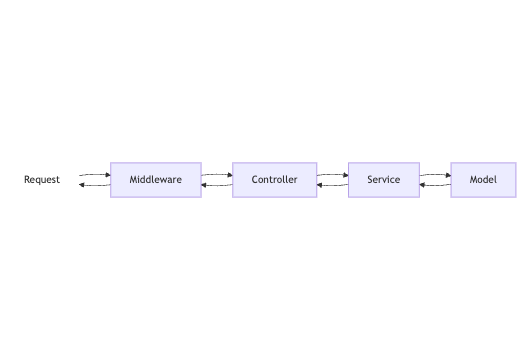
\includegraphics[width=0.88\textwidth]{Images/MVCS.png}
\caption{Minh họa kiến trúc phía máy chủ (MVCS) sau khi SSH và triển khai mã nguồn backend trên EC2.}
\label{fig:deploy-ec2-ssh}
\end{figure}

\subsection{Clone mã nguồn, Prisma, chạy API}

\begin{itemize}
    \item \texttt{git clone} kho SoCo-DATN (monorepo).
    \item \texttt{cd database \&\& npm install}; \texttt{cd ../backend \&\& npm install}.
    \item Tạo \texttt{backend/.env}: \texttt{DATABASE\_URL}, \texttt{REDIS\_URL}, \texttt{JWT\_SECRET}, \texttt{SENSITIVE\_DATA\_KEY}, \texttt{FRONTEND\_URL} (sau có URL Vercel), Cloudinary/SMTP/AI nếu cần.
    \item Chạy:
\begin{lstlisting}[language=bash]
cd backend
npm run prisma:generate
npm run prisma:migrate:deploy
NODE_ENV=production pm2 start src/server.js --name soco-api
pm2 save
pm2 startup
\end{lstlisting}
    \item Sau khi có URL API HTTPS: dùng \texttt{https://.../api} cho \texttt{VITE\_API\_BASE\_URL} trên Vercel; cập nhật \texttt{FRONTEND\_URL} trên server $\rightarrow$ \texttt{pm2 restart soco-api}.
\end{itemize}

%----------------------------------------------------------------------
\section{Triển khai front-end trên Vercel}
%----------------------------------------------------------------------

\subsection{Cấu hình project}

\begin{itemize}
    \item Đăng nhập \href{https://vercel.com}{vercel.com} (thường qua GitHub).
    \item \textit{Add New $\rightarrow$ Project} $\rightarrow$ import repo chứa SoCo-DATN.
    \item \textbf{Root Directory}: chọn \texttt{frontend}.
    \item \textbf{Build Command}: \texttt{npm run build}.
    \item \textbf{Output Directory}: \texttt{dist}.
    \item \textbf{Install Command}: \texttt{npm install} (hoặc \texttt{npm ci} nếu nhóm dùng lockfile thống nhất).
\end{itemize}





\subsection{Biến môi trường và deploy}

\begin{itemize}
    \item \textit{Settings $\rightarrow$ Environment Variables}: thêm \texttt{VITE\_API\_BASE\_URL} = URL API HTTPS có \texttt{/api}.
    \item \textit{Deploy}; khi xong, copy URL dạng \texttt{https://<ten>.vercel.app}.
    \item Cập nhật \texttt{FRONTEND\_URL} trên EC2 khớp URL Vercel (hoặc domain custom) $\rightarrow$ restart PM2.
    \item Push lên nhánh đã liên kết $\rightarrow$ Vercel có thể tự build lại (xem tab Deployments).
\end{itemize}



\begin{figure}[H]
\centering
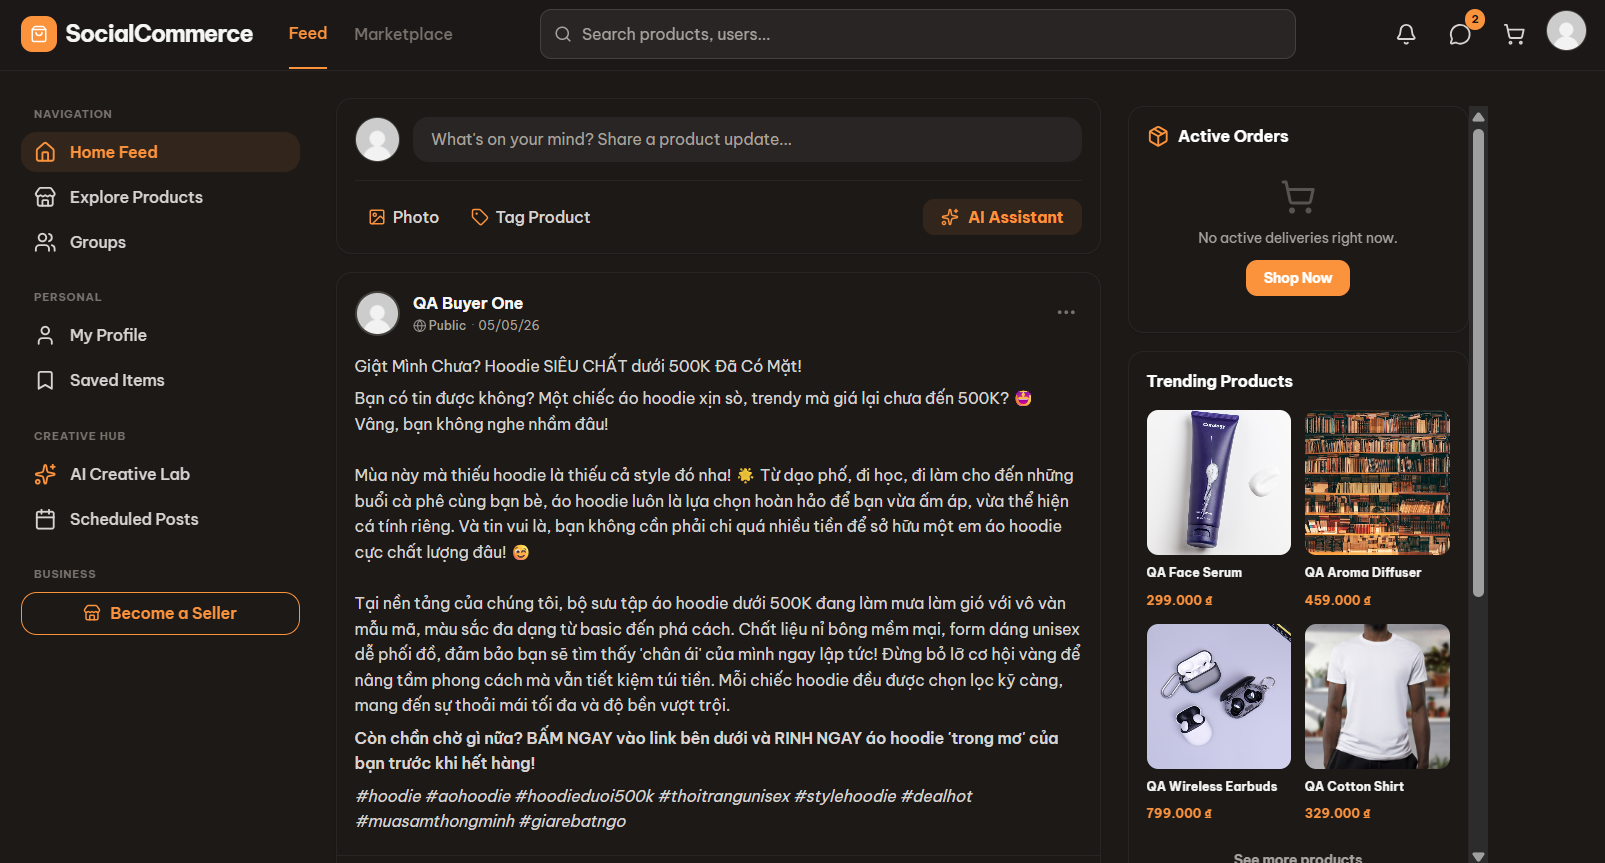
\includegraphics[width=\textwidth]{Images/UI/module2/home-feed.png}
\caption{Minh họa kết quả: giao diện người dùng (bảng tin) sau khi ứng dụng được triển khai và truy cập qua URL công khai.}
\label{fig:deploy-vercel-success}
\end{figure}

%----------------------------------------------------------------------
\section{Backend quản trị và giao diện admin}
%----------------------------------------------------------------------

\begin{itemize}
    \item \textbf{admin/backend}: tiến trình Node riêng (ví dụ PM2 thứ hai), cổng mặc định 5001; \texttt{DATABASE\_URL} trùng Neon; \texttt{ADMIN\_JWT\_SECRET}; \texttt{ADMIN\_CORS\_ORIGIN} khớp origin frontend admin.
    \item \textbf{admin/frontend}: có thể tạo thêm project Vercel, Root \texttt{admin/frontend}; \texttt{VITE\_ADMIN\_API\_BASE\_URL}, \texttt{VITE\_CORE\_PUBLIC\_URL} (xem \texttt{admin/README.md}, \texttt{.env.example}).
\end{itemize}

%----------------------------------------------------------------------
\section{Kết quả và checklist}
%----------------------------------------------------------------------

\subsection{Sau khi hoàn tất}

\begin{itemize}
    \item Mở được SPA từ Vercel; REST và Socket.IO tới EC2 qua HTTPS/WSS.
    \item Dữ liệu trên Neon; Redis hoạt động nếu đã cấu hình.
    \item Ghi vào báo cáo: URL frontend production, URL kiểm tra \texttt{/health} (ví dụ \texttt{https://api.../health}).
\end{itemize}

\subsection{Checklist production}

\begin{itemize}
    \item \texttt{NODE\_ENV=production}; không commit \texttt{.env}.
    \item TLS cho API; \texttt{FRONTEND\_URL} và \texttt{VITE\_*} đúng domain công khai.
    \item Đã chạy migration trên Neon; thử đăng nhập, upload Cloudinary, SMTP, AI (nếu bật).
    \item Rà soát Security Group; hạn chế SSH mở rộng \texttt{0.0.0.0/0} nếu có thể.
\end{itemize}
